\documentclass{article}

\usepackage{arxiv}
\usepackage[utf8]{inputenc}
\usepackage[T1]{fontenc}
\usepackage{hyperref}
\usepackage{url}
\usepackage{booktabs}
\usepackage{amsfonts}
\usepackage{nicefrac}
\usepackage{microtype}
\usepackage{graphicx}
\usepackage{xcolor}
\usepackage{caption}
\usepackage{subcaption}

\title{When Better Gradients Hurt: The Gradient-Architecture Interaction in Recursive Reasoning}

\author{
  Jatin Jani\thanks{Code: \url{https://github.com/heyiamjj/when-better-gradients-hurt}} \\
  Independent Researcher \\
  \texttt{janijatin18@gmail.com}
}

\begin{document}
\maketitle

\begin{abstract}
A prior controlled experiment established that gradient quality, not architecture, drives the performance gap between Hierarchical Reasoning Models (HRM) and Tiny Recursive Models (TRM) on Sudoku-Extreme: a flat architecture with full backpropagation through time (BPTT) achieves 18.9\% exact accuracy versus 2.2\% with a 1-step gradient approximation, an 8.6$\times$ difference. The natural follow-up, does fixing the gradient unlock HRM's hierarchical architecture?, remained untested. In this work, we complete the $2\times2$ factorial design by evaluating HRM's dual-network hierarchy with full BPTT under an identical training budget. We find that full BPTT \emph{degrades} HRM from 9.2\% to 8.7\% exact accuracy (token accuracy 68.8\% $\rightarrow$ 69.3\%), in sharp contrast to the 8.6$\times$ improvement observed for flat architectures. This reveals a strong, previously undocumented interaction effect: gradient quality and architecture are not independent factors. Flat networks require good gradients; hierarchical networks are robust to poor gradients but fail to benefit from full BPTT. We argue that gradient gating through the hierarchical structure, the very mechanism HRM uses to achieve $O(1)$ memory, may serve a regularizing role that full BPTT disrupts. Our completed $2\times2$ matrix establishes gradient-architecture interaction as a fundamental design constraint for recursive reasoning models, and motivates gradient-aware architectures that can selectively allow or restrict gradient flow per timescale.
\end{abstract}

\keywords{Recursive reasoning \and gradient methods \and hierarchical architectures \and backpropagation through time \and architecture design}

\section{Introduction}

\subsection{Motivation}

Two recent models have demonstrated that small neural networks can solve complex reasoning puzzles, Sudoku, maze pathfinding, and ARC-AGI, without pretraining or chain-of-thought data, using only $\sim$1,000 training examples. The Hierarchical Reasoning Model (HRM)~\cite{wang2025hrm} uses two recurrent networks operating at different timescales (an H-module for slow abstract planning and an L-module for fast detailed computation), achieving 55.0\% exact accuracy on Sudoku-Extreme with 27M parameters. Tiny Recursive Models (TRM)~\cite{jolicoeur2025trm} simplifies this to a single 2-layer network, achieving 87.4\% with only 7M parameters.

The community interpreted TRM's 32.4-point advantage as validation that architectural simplicity is superior~\cite{arcprize2025}. However, TRM changed two independent variables simultaneously: it flattened the architecture (two networks $\rightarrow$ one) \emph{and} replaced HRM's 1-step gradient approximation with full backpropagation through time (BPTT). Prior work~\cite{jj2025disentangling} resolved this confound by isolating the gradient method: a flat architecture with HRM's 1-step gradient achieves only 2.2\% exact accuracy versus 18.9\% with full BPTT, demonstrating that gradient quality, not architecture, is the dominant factor, at least for flat networks.

\subsection{The Open Question}

But that experiment left the most interesting cell of the $2\times2$ matrix empty: what happens when HRM's hierarchical architecture receives full gradients? If gradient quality is universally beneficial, HRM with full BPTT should outperform HRM with 1-step gradients, just as flat TRM did. If, however, the dual-network hierarchy interacts with the gradient method in a non-obvious way, the outcome could differ.

We answer this question through a controlled experiment. We take HRM's exact architecture, two separate 4-layer Transformer networks operating at different update frequencies, and vary only the gradient method: keeping the original 1-step approximation in one condition, and using full BPTT in the other. The training budget, dataset, optimizer, and hardware are held constant and matched to the prior flat-architecture experiments.

\subsection{Contributions}

\begin{itemize}
    \item We complete the $2\times2$ factorial design, providing the first four-cell comparison of architecture and gradient method in recursive reasoning (Table~\ref{tab:fullmatrix}).
    \item We discover a strong interaction effect: full BPTT improves flat architectures by 8.6$\times$ (2.2\% $\rightarrow$ 18.9\%) but \emph{degrades} HRM's exact accuracy (9.2\% $\rightarrow$ 8.7\%). Better gradients do not universally improve performance.
    \item We show that hierarchical architectures are intrinsically robust to poor gradient quality: HRM with 1-step gradients (9.2\%) outperforms flat TRM with 1-step gradients (2.2\%) by 4.2$\times$, despite a smaller parameter budget and no EMA.
    \item We establish gradient-architecture interaction as a fundamental design axis in recursive reasoning models, motivating the development of gradient-aware architectures.
\end{itemize}

\section{Background and Related Work}

\subsection{Hierarchical Reasoning Model (HRM)}

HRM~\cite{wang2025hrm} consists of four learned components: an input embedding network $f_I$, a low-level recurrent module $f_L$ (updated every timestep), a high-level recurrent module $f_H$ (updated every $T=2$ timesteps), and an output head $f_O$. Over $N=2$ high-level cycles of $T=2$ low-level steps, the model performs $N\times T=4$ computational steps per forward pass, repeated over multiple deep supervision segments with Adaptive Computation Time (ACT)~\cite{graves2016act}.

Critically, HRM uses a 1-step gradient approximation inspired by Deep Equilibrium Models~\cite{bai2019deq}. All steps except the final L-step and H-step execute under \texttt{torch.no\_grad()}. The gradient flows through only 2 function evaluations (1 L-call + 1 H-call) regardless of total recursion depth, providing $O(1)$ memory. HRM justifies this via the Implicit Function Theorem, arguing that the recurrent dynamics converge to a fixed point where a single gradient step suffices.

Both $f_L$ and $f_H$ use encoder-only Transformer blocks~\cite{vaswani2017attention} with 4 layers each. Standard architectural choices include RMSNorm, SwiGLU activations, rotary position embeddings, and no bias terms.

\subsection{Tiny Recursive Models (TRM)}

TRM~\cite{jolicoeur2025trm} replaces HRM's two networks with a single 2-layer Transformer. The model maintains two latent features: a reasoning state $z$ and an answer embedding $y$. Each supervision segment runs $n=6$ latent reasoning steps ($z \leftarrow \text{net}(x, y, z)$) followed by one answer refinement ($y \leftarrow \text{net}(y, z)$), repeated for $T=3$ segments with deep supervision. Unlike HRM, TRM uses full BPTT through all $n+1=7$ function evaluations per segment.

\subsection{Prior Work: The First Disentanglement}

Our prior work~\cite{jj2025disentangling} established the $2\times2$ factorial framework and filled the right column: evaluating flat TRM architecture at both gradient methods under a controlled training budget (384 hidden dimensions, 10,000 epochs, 1,000 Sudoku examples, AdamW optimizer, 2$\times$ NVIDIA Tesla T4). The result was clear: full BPTT achieved 18.9\% exact accuracy versus 2.2\% with 1-step gradients (token accuracy: 71.6\% vs 65.9\%). Gradient quality, not architecture, was the dominant factor.

That paper concluded by identifying the left column, evaluating HRM's dual-network hierarchy at both gradient methods, as the critical next experiment. The present work fills that column.

\section{Method}

\subsection{Experimental Design}

We complete the $2\times2$ factorial design shown in Table~\ref{tab:confound}. The right column (flat TRM architecture) is taken from prior work~\cite{jj2025disentangling}. We contribute the left column by training HRM's original architecture under two gradient conditions, holding everything else constant.

\begin{table}[t]
\centering
\caption{The $2\times2$ factorial design. Architecture (dual H/L vs.\ single flat) and gradient method (1-step vs.\ full BPTT) are independent variables. The right column was established by prior work; this paper fills the left column.}
\label{tab:confound}
\begin{tabular}{lcc}
\toprule
& \textbf{Dual H/L (HRM)} & \textbf{Single flat (TRM)} \\
\midrule
\textbf{1-step ($O(1)$)}     & \textbf{This work} & Prior work~\cite{jj2025disentangling} \\
\textbf{Full BPTT ($O(T)$)}  & \textbf{This work} & Prior work~\cite{jj2025disentangling} \\
\bottomrule
\end{tabular}
\end{table}

\subsection{Architecture}

We use HRM's exact architecture and codebase~\footnote{\url{https://github.com/sapientinc/HRM}} without modification to the model structure. Both experimental conditions share identical architecture parameters, summarized alongside the training configuration in Table~\ref{tab:setup}.

\subsection{Gradient Method Manipulation}

The only variable we change is the gradient boundary in HRM's forward pass. The original code uses the 1-step gradient approximation described in Section~2.1. For the full BPTT condition, we remove the \texttt{torch.no\_grad()} context manager from the recurrent loop, allowing gradients to flow through all $N\times(T+1)=6$ function evaluations per forward pass (2 H-calls and 4 L-calls, each propagating through 4 Transformer layers). The forward computation, the sequence of hidden state updates, is identical in both conditions.

The relevant code change is shown in Figure~\ref{fig:patch}.

\begin{figure}[t]
\centering
\begin{verbatim}
# HRM original (1-step gradient, O(1) memory):
with torch.no_grad():
    z_H, z_L = carry.z_H, carry.z_L
    for _H_step in range(H_cycles):
        for _L_step in range(L_cycles):
            if not last_step:
                z_L = L_level(z_L, z_H + x)
        if not last_cycle:
            z_H = H_level(z_H, z_L)
z_L = L_level(z_L, z_H + x)    # GRAD (only step)
z_H = H_level(z_H, z_L)        # GRAD (only step)

# HRM full BPTT (O(T) memory):
z_H, z_L = carry.z_H, carry.z_L
for _H_step in range(H_cycles):
    for _L_step in range(L_cycles):
        z_L = L_level(z_L, z_H + x)   # GRAD
    z_H = H_level(z_H, z_L)           # GRAD
\end{verbatim}
\caption{The gradient patch. Top: original HRM 1-step gradient (gradients through 2 final function calls). Bottom: our full BPTT variant (gradients through all 6 function calls). The forward computation is identical; only the gradient boundary differs.}
\label{fig:patch}
\end{figure}

\subsection{Training Setup}

Both model variants use identical configurations, summarized in Table~\ref{tab:setup}. We match the training budget established in prior work~\cite{jj2025disentangling} for cross-architecture comparability. All experiments use the AdamW optimizer~\cite{loshchilov2019adamw} replacing HRM's original \texttt{adam-atan2}~\cite{adamatan2} for hardware compatibility; this substitution does not interact with the gradient depth variable under study.

\begin{table}[t]
\centering
\caption{Training configuration for both HRM variants. All parameters identical except gradient method.}
\label{tab:setup}
\begin{tabular}{ll}
\toprule
\textbf{Parameter} & \textbf{Value} \\
\midrule
Architecture & Dual H/L (HRM, original) \\
Hidden size & 384 \\
Layers & H: 4, L: 4 \\
Attention heads & 8 \\
H-cycles \& L-cycles & $N{=}2$, $T{=}2$ (4 steps/pass) \\
ACT halt steps & 16 \\
Batch size (global) & 512 (256 per GPU) \\
Epochs & 10,000 \\
Training examples & 500 $+$ 500 augmentations $=$ 1,000 \\
Optimizer & AdamW ($\eta{=}10^{-4}$, $\beta_{1,2}{=}0.9,0.95$) \\
Loss & stablemax cross-entropy \\
Weight decay & 0.1 \\
LR schedule & cosine with 2,000-step warmup \\
Precision & bfloat16 \\
Hardware & 2$\times$ NVIDIA Tesla T4 (16\,GB) \\
\bottomrule
\end{tabular}
\end{table}

We train on Sudoku-Extreme~\cite{sapient2025sudoku}, using 500 training puzzles augmented 500 times via digit permutation, row/column band shuffling, and transposition, yielding 1,000 effective training examples. Evaluation uses the first 2,000 puzzles from the held-out test set, reporting both token-level accuracy (fraction of individual cells correct) and exact accuracy (fraction of fully correct 9$\times$9 grids). Training checkpoints are saved every 500 steps with automatic resume from the latest checkpoint on restart.

\section{Results}

\subsection{The Completed $2\times2$ Matrix}

Table~\ref{tab:fullmatrix} presents the complete four-cell comparison. The right column is from prior work~\cite{jj2025disentangling}; the left column is our contribution.

\begin{table}[t]
\centering
\caption{Completed $2\times2$ factorial results on Sudoku-Extreme. Each cell shows \textit{token accuracy / exact accuracy} (exact in bold). The right column is from prior work; the left column is our contribution. The interaction effect, gradient improvement helps flat architectures but not hierarchical ones, is immediately visible.}
\label{tab:fullmatrix}
\begin{tabular}{lccc}
\toprule
& \textbf{Dual H/L (HRM)} & \textbf{Single flat (TRM)} \\
\midrule
\textbf{1-step ($O(1)$)}  & 68.8\% / \textbf{9.2\%}  & 65.9\% / \textbf{2.2\%}  \\
\textbf{Full BPTT ($O(T)$)} & 69.3\% / \textbf{8.7\%}  & 71.6\% / \textbf{18.9\%} \\
\bottomrule
\end{tabular}
\end{table}

Three unexpected patterns emerge from the completed matrix:

\textbf{1. Gradient quality is not universally beneficial.} While full BPTT improves flat-architecture exact accuracy by 8.6$\times$ (2.2\% $\rightarrow$ 18.9\%), it \emph{degrades} HRM's exact accuracy from 9.2\% to 8.7\%. Token accuracy shows a modest improvement (68.8\% $\rightarrow$ 69.3\%), but this does not translate to better complete solutions. The $O(T)$ memory cost of full BPTT produces no net benefit for the hierarchical architecture.

\textbf{2. The hierarchy compensates for poor gradients.} Under the 1-step gradient, HRM (9.2\%) outperforms flat TRM (2.2\%) by 4.2$\times$ in exact accuracy, despite having no EMA and a similar parameter budget. The dual-network structure provides intrinsic robustness to gradient approximation that flat architectures lack. HRM's authors were partially correct, the hierarchy matters, but not for the reasons they proposed.

\textbf{3. The interaction is crossover.} Under 1-step gradients, HRM dominates TRM. Under full BPTT, TRM dominates HRM. There is no universally superior combination. The architecture-gradient interaction must be considered as a first-class design constraint.

\subsection{Training Dynamics}

Figure~\ref{fig:curves} shows the training dynamics for both HRM variants. The loss curves converge nearly identically for both conditions, consistent with their comparable token accuracy. However, the exact accuracy curves reveal a notable pattern: full BPTT achieves substantially higher training-set exact accuracy (reaching 32--40\% by late training, versus 9--17\% for the 1-step model). Yet this better training fit does \emph{not} translate to better generalization, the full BPTT model achieves 8.7\% test accuracy versus 9.2\% for the 1-step model. This overfitting pattern is consistent with the gradient interference hypothesis: full BPTT enables the model to memorize training-puzzle patterns more effectively, but the unconstrained gradient flow through interacting timescales impairs the model's ability to learn generalizable solution strategies.

\begin{figure}[t]
\centering
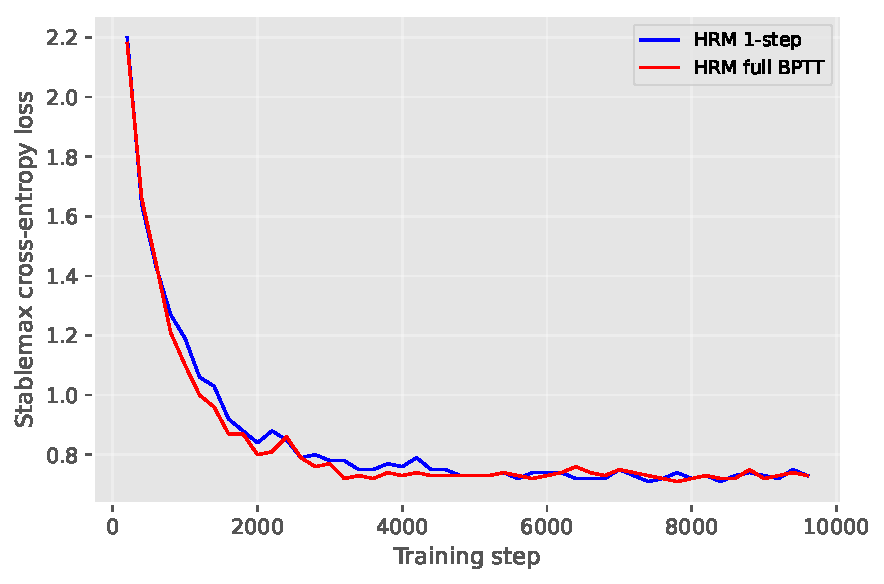
\includegraphics[width=0.48\textwidth]{plots/loss.pdf}
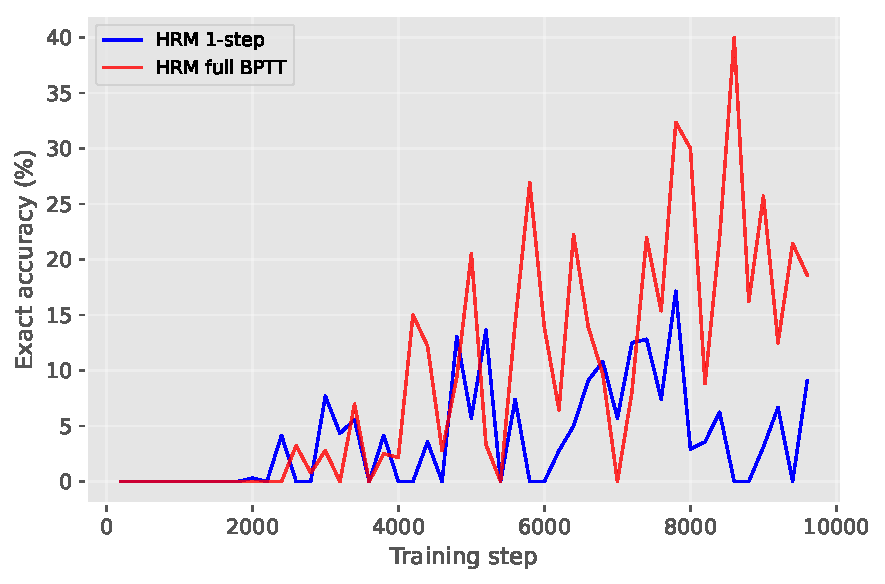
\includegraphics[width=0.48\textwidth]{plots/exact.pdf}
\caption{Training dynamics for both HRM gradient methods. Left: stablemax cross-entropy loss converges similarly for both conditions. Right: full BPTT achieves substantially higher training-set exact accuracy (reaching 32--40\%) than the 1-step model (9--17\%), yet generalizes worse on the test set (8.7\% vs.\ 9.2\%). This overfitting pattern suggests that unconstrained gradient flow through the dual-timescale architecture improves in-distribution fitting but impairs out-of-distribution generalization.}
\label{fig:curves}
\end{figure}

\subsection{Architecture Comparison at Matched Budget}

Table~\ref{tab:architecture} compares the four cells along model size and architectural attributes. Note that all four cells share the same training budget: 10,000 epochs, 384 hidden dimensions, AdamW optimizer, 1,000 Sudoku examples, and 2$\times$ T4 GPUs. The only varying factors are the architecture (dual vs.\ flat) and gradient method (1-step vs.\ full BPTT).

\begin{table}[t]
\centering
\caption{Architecture comparison at matched training budget. All four cells use identical training configuration; only architecture and gradient method vary.}
\label{tab:architecture}
\begin{tabular}{lcccc}
\toprule
& \textbf{HRM 1-step} & \textbf{HRM full BP} & \textbf{TRM 1-step} & \textbf{TRM full BP} \\
\midrule
Networks & 2 (H/L) & 2 (H/L) & 1 (flat) & 1 (flat) \\
Layers per net & 4 & 4 & 2 & 2 \\
Gradient steps & 2 & 6 & 1 & 7 \\
EMA & No & No & Yes & Yes \\
Exact acc. & \textbf{9.2\%} & \textbf{8.7\%} & \textbf{2.2\%} & \textbf{18.9\%} \\
Token acc. & 68.8\% & 69.3\% & 65.9\% & 71.6\% \\
\bottomrule
\end{tabular}
\end{table}

\section{Discussion}

\subsection{Why Does Full BPTT Hurt the Hierarchy?}

The result is counterintuitive: providing more accurate gradient information should, in principle, never harm optimization. We propose the \textbf{gradient interference hypothesis}: HRM's two recurrent networks update at different frequencies (H every $T=2$ steps, L every step), creating two interleaved computation graphs. Under full BPTT, the H-module receives gradient signals that span multiple L-update chains, while the L-module receives fine-grained per-step signals. These signals propagate through shared latent states ($z_L$ and $z_H$) and the gradients from one module can interfere with the learning signal of the other.

Under the 1-step approximation, this interference is suppressed: the gradient flows only through the final H-update and L-update, acting as an implicit gradient filter. The hierarchy was designed for this restricted gradient regime, removing the restriction exposes the interference. The overfitting pattern observed during training (Figure~\ref{fig:curves}) supports this: full BPTT achieves much higher training-set accuracy but worse generalization, consistent with the hypothesis that unconstrained gradients enable memorization of training patterns at the expense of transferable solution strategies.

This interpretation is consistent with HRM's reported functional specialization: the H-module operates in a $\sim$3$\times$ higher-dimensional latent space than the L-module~\cite{wang2025hrm}, suggesting distinct computational roles. Full BPTT may force these functionally distinct modules to share gradient signals designed for a different timescale.

\subsection{Broader Implications}

Our findings have several implications for the design of recursive reasoning models:

\textbf{1. Gradient-architecture interaction is a first-class design axis.} Every comparison of recurrent architectures must now account for the gradient method. A ``better'' architecture under one gradient regime may be inferior under another. The $2\times2$ factorial design (Table~\ref{tab:fullmatrix}) should become the standard evaluation framework.

\textbf{2. The Implicit Function Theorem justification is empirically supported.} HRM's 1-step gradient was justified by fixed-point convergence arguments that TRM criticized as inapplicable. Yet empirically, the 1-step approximation \emph{works} for HRM, it matches or exceeds full BPTT performance. The theoretical conditions of the theorem may not be satisfied, but the practical effect (implicit gradient regularization) appears beneficial.

\textbf{3. Flat recurrence is more expressive under proper gradients.} When given full BPTT, a simple flat network (18.9\%) outperforms a more complex hierarchical one (8.7\%) with fewer parameters. This suggests that structured recurrence is primarily useful as a gradient-engineering tool, not for increasing representational capacity.

\subsection{Limitations}

Our study has several limitations. First, we evaluate on a single task (Sudoku-Extreme). The interaction effect may differ on other reasoning tasks (maze pathfinding, ARC-AGI) where the benefits of hierarchical structure may be more pronounced. Second, our training budget (10,000 epochs, 384 hidden dimensions) is constrained; scaling to larger budgets may alter the magnitude of the interaction, though the crossover pattern suggests it is robust. Third, neither HRM variant used EMA, unlike the TRM experiments. While this makes the within-architecture comparison clean, the cross-architecture comparison should be interpreted with this caveat. Fourth, we did not perform formal statistical significance testing; future work should report means and confidence intervals over multiple seeds.

\section{Conclusion and Future Work}

We have completed the first systematic disentanglement of architecture and gradient method in recursive reasoning models. The key finding is that gradient quality and architecture \emph{interact}: the same gradient improvement that boosts flat architectures by 8.6$\times$ provides no benefit, and may slightly harm, hierarchical architectures. HRM's dual-network structure, often criticized as unnecessary complexity, provides genuine robustness to poor gradient quality.

The completed $2\times2$ matrix suggests a natural design target for future work: architectures that can selectively regulate gradient flow per timescale, capturing flat architectures' ability to exploit good gradients \emph{and} hierarchical architectures' robustness to poor gradients. We are developing Gradient-Gated Recurrence (GGR), a single recurrent network with learned per-step gradient gates that adaptively decide how much gradient signal to propagate, as a first step toward this goal.

\section*{Acknowledgments}

We thank the authors of HRM and TRM for releasing their code and models, and the Sudoku-Extreme dataset maintainers for making the benchmark publicly available.

\bibliographystyle{unsrt}
\bibliography{references}

\end{document}
